\chapter {Implémentation de l'algorithme}
\section*{Introduction}
Dans ce chapitre, nous expliquons l'environnement de travail que nous avons utilisé afin d'implémenter CBSO, puis nous présentons l'interface graphique de notre application.\\

\section{Outils de travail}
Nous avons eu besoin des outils suivants:

\begin{itemize}
	\item langage de programmation Java,
	\item environnement de développement Netbeans,
	\item machine dotée d'un processeur Intel core i3 et d'une RAM de 4GO. 
\end{itemize}

\bigskip

\section{Application}
L'interface graphique de notre application aide l'utilisateur à paramétrer l'algorithme et à l'exécuter sur les différentes fonctions de test.

Les paramètres de l'algorithme sont chargés automatiquement à l'apparition de l'interface graphique, ils peuvent être changés par l'utilisateur.\\\\
\bigskip\bigskip\bigskip
\vspace{6em}

Les figures suivantes montrent l'interface graphique avec les différentes étapes d'utilisation.

\begin{figure}[H]
	\centering
	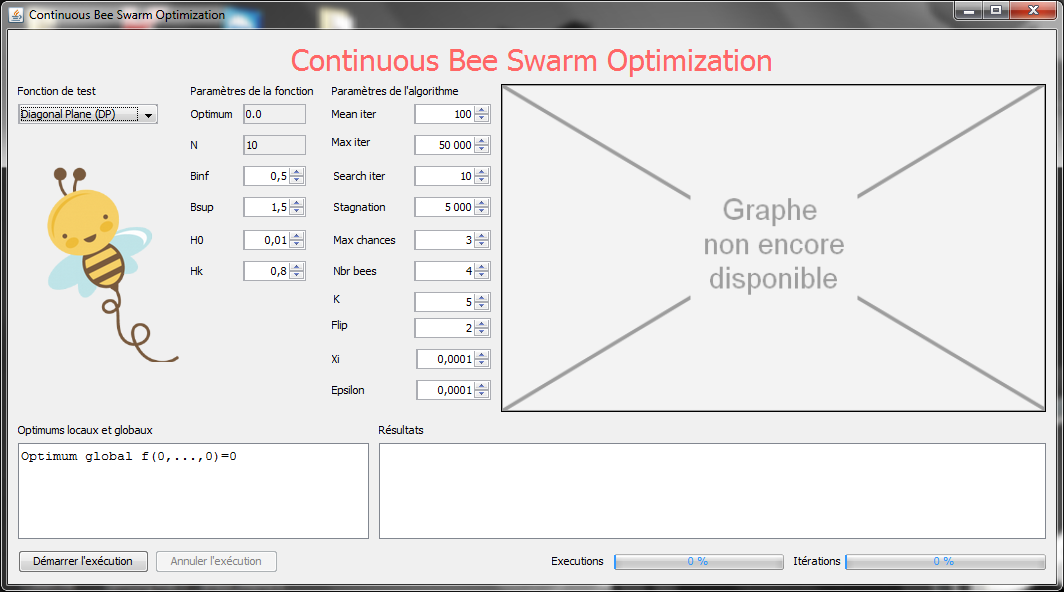
\includegraphics[width=\textwidth,keepaspectratio]{IHM1}
	\caption{Interface graphique de l'application}
\end{figure}

\bigskip \bigskip 
Il suffit que l'utilisateur passe le curseur sur le nom d'un paramètre pour qu'une information explicative de ce dernier apparaisse.\\\\


\begin{figure}[H]
	\centering
	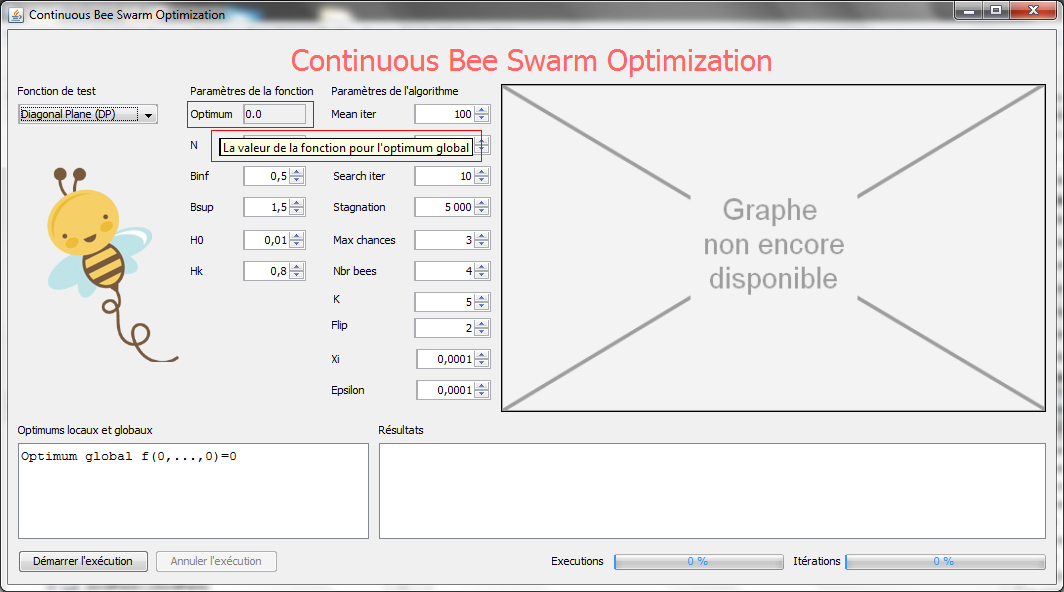
\includegraphics[width=\textwidth,keepaspectratio]{IHM2}
	\caption{Explication des paramètres de l'algorithme}
\end{figure}

\bigskip \bigskip \bigskip 

L'utilisateur commence  par choisir la fonction de test à partir de la liste déroulante qui se trouve en haut à gauche de l'interface.

\begin{figure}[H]
	\centering
	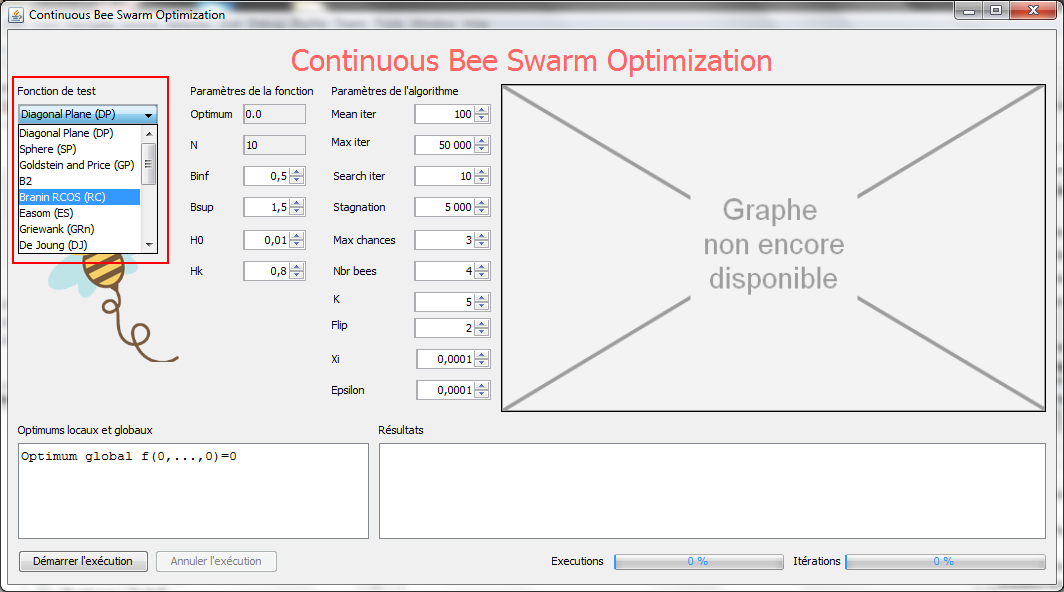
\includegraphics[width=\textwidth,keepaspectratio]{IHM3}
	\caption{Choix de la fonction de test}
\end{figure}
\vspace{-2em}
Après avoir choisi la fonction, ses paramètres sont chargés automatiquement. L'utilisateur peut choisir de travailler sur un sous-domaine du domaine de définition de la fonction comme il peut changer les paramètres $h_0$ et $h_k$.

\begin{figure}[H]
	\centering
	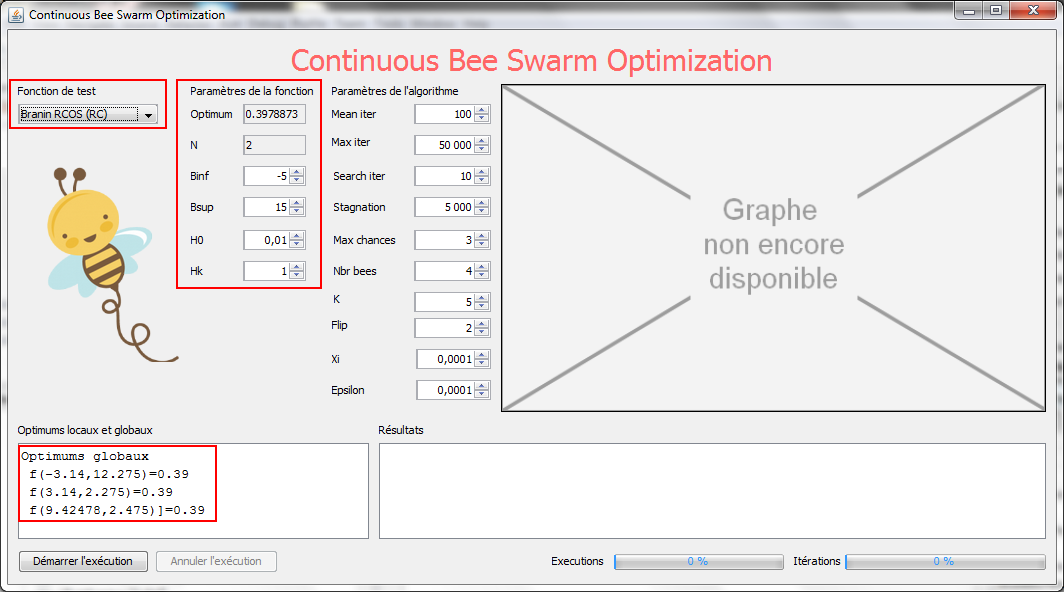
\includegraphics[width=\textwidth,keepaspectratio]{IHM4}
	\caption{Chargement des paramètres de la fonction de test}
\end{figure}
\vspace{-2em}
Avant de lancer CBSO, l'utilisateur peut fixer le nombre d'exécutions indépendantes de l'algorithme à travers le paramètre $MeanIter$. Nous avons fixé par défaut ce nombre à $100$ itérations indépendantes et cela pour avoir des résultats plus fiables.

L'utilisateur peut alors lancer CBSO en appuyant sur le bouton \emph{Démarrer l'exécution}. La progression de l'algorithme est observée à travers deux barres de progression, la première indiquant le numéro de l'exécution courante et la deuxième le numéro d'itération courante dans l'exécution.


\begin{figure}[H]
	\centering
	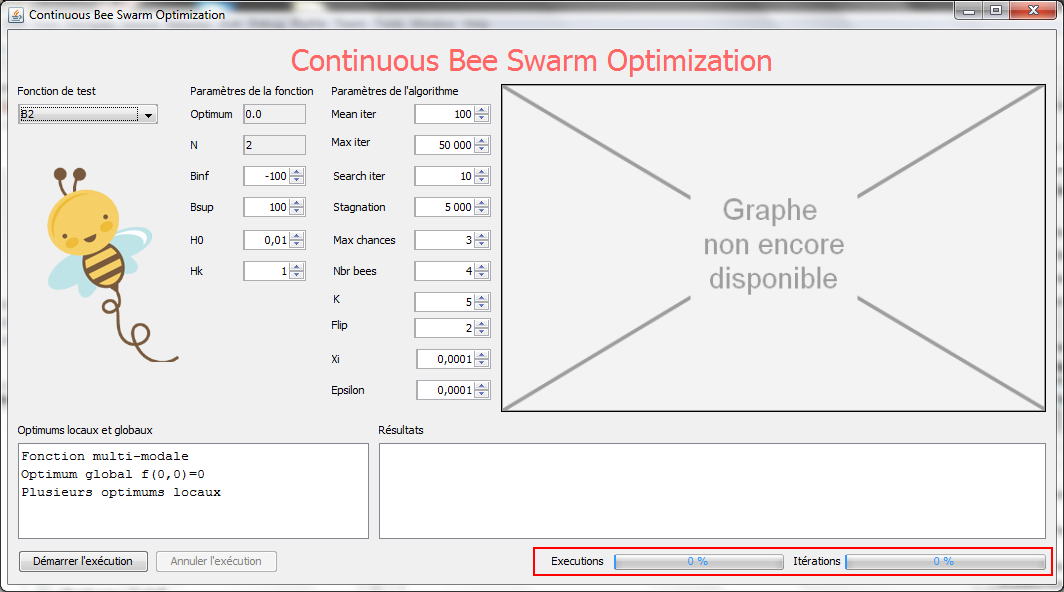
\includegraphics[width=\textwidth,keepaspectratio]{IHM5}
	\caption{Barres de progression}
\end{figure}

Dans le cas où l'utilisateur veut interrompre l'exécution, il appuie sur le bouton \emph{Annuler l'exécution}.
\begin{figure}[H]
	\centering
	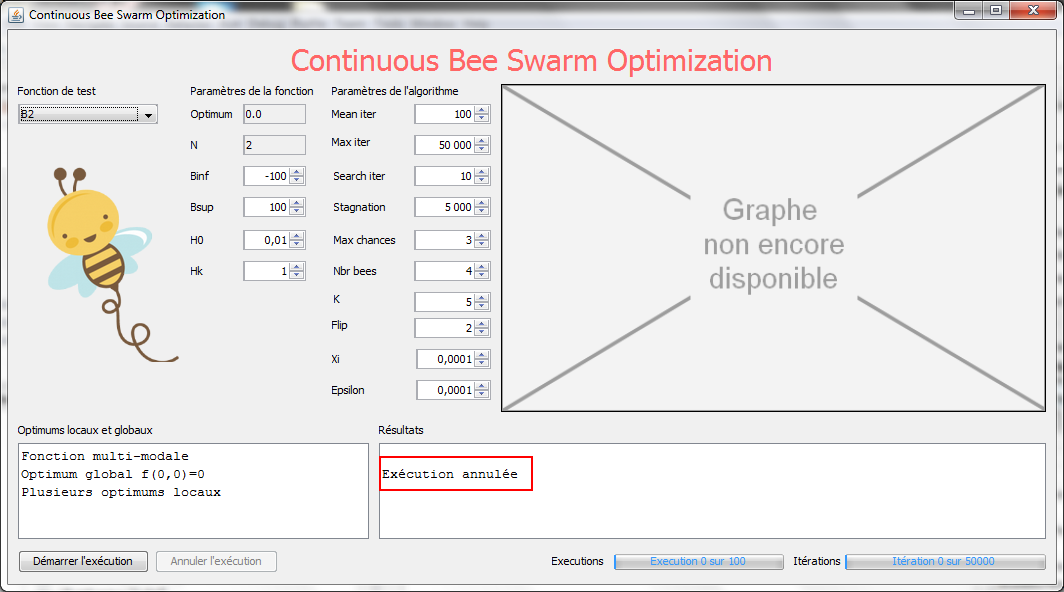
\includegraphics[width=\textwidth,keepaspectratio]{IHM6}
	\caption{Annulation de l'exécution}
\end{figure}

A la fin de l'algorithme, les informations concernant l'exécution sont affichées dans la zone de texte en bas à droite. Ces informations comportent la meilleure solution trouvée, le nombre des itérations, le nombre des évaluations de la fonction, le taux de réussite, de stagnation et d'atteinte de $MaxIter$ ainsi que le temps d'exécution.

\vspace{0.5em}

De plus, un graphe est affiché représentant l'évolution de l'évaluation du sommet de référence à travers les 3000 premières itérations au maximum de la dernière exécution.

\begin{figure}[H]
	\centering
	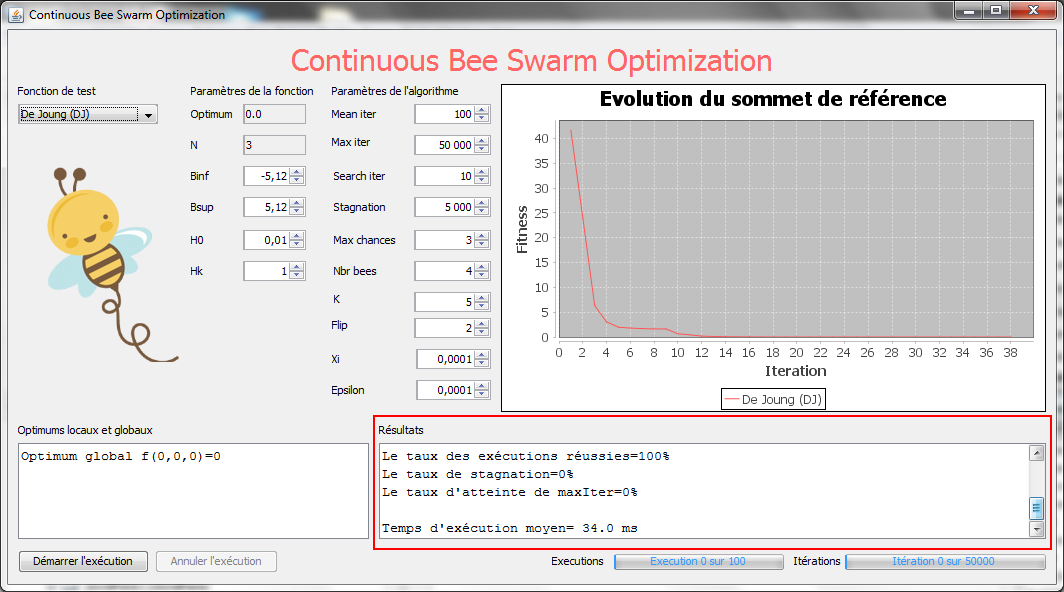
\includegraphics[width=\textwidth,keepaspectratio]{IHM7}
	\caption{Affichage des résultats}
\end{figure}

\section*{Conclusion}
Après avoir présenté l'interface graphique de l'application, l'étape suivante est celle du test et de l'évaluation de CBSO.
